\documentclass[10pt]{beamer}
% \setbeamercovered{transparent}
\beamerdefaultoverlayspecification{<+(1)-| alert@+(1)>}
\usetheme{Boadilla}
\usecolortheme{seahorse}
\usefonttheme{structurebold}
\usepackage{multicol}
\usepackage{graphicx}
\usepackage{tikz}
\usepackage{calc}
\usetikzlibrary{calc}
\usepackage{fp}
\usepackage{listings} % Pacote para destacar código fonte
\usepackage{amsmath} 
\usepackage{amssymb} 
\usepackage{helvet}
\usepackage{xcolor}
\usepackage{pgfplots}
\usepackage{array}
\usepackage{arydshln}
\usepackage{enumitem}
\pgfplotsset{compat=1.18}
\setlist[itemize]{label=\textbullet}

\lstset{
  language=C++,
  basicstyle=\small\ttfamily,
  numbers=left, 
  numberstyle=\tiny, 
  stepnumber=1, 
  numbersep=-30pt, 
}

\newcommand{\codecppNoTitle}[2][0.6]{
  \centering
  \begin{minipage}{#1\textwidth}
    %Referencia: https://ctan.dcc.uchile.cl/macros/latex/contrib/listings/listings.pdf
    \lstset{
      language=C++,
      numbers=left,
      numberstyle=\tiny,
      stepnumber=1,
      numbersep=5pt,
      showstringspaces = false,
      frame=shadowbox,
      commentstyle=\color{commentgreen},
      keywordstyle=\color{eminence},
      stringstyle=\color{red},
      backgroundcolor=\color{black!3},
      keywordstyle=\color{blue},
      rulesepcolor=\color{black!5},
      basicstyle=\small\ttfamily, % basic font setting
      emph={int,char,double,float,unsigned,void,bool},
      emphstyle={\color{blue}}
    }
    \lstinputlisting{#2}
  \end{minipage}}


% Definindo as cores para as palavras reservadas
\definecolor{keywordblue}{RGB}{0,0,255}
\definecolor{identifierblack}{RGB}{0,0,0}

\newcommand{\duascolunas}[2]{
  \begin{columns}
    \begin{column}{0.72\textwidth}
      #1
    \end{column}
    \begin{column}{0.28\textwidth}
		#2
	\end{column}
  \end{columns}
}

\title{Análise de Complexidade}
\author{Prof. Kennedy Reurison Lopes}
\subtitle{Parte 3}
\date{\today}

% Início do documento
\begin{document}

\frame{\titlepage}% Parte 3
\begin{frame}[t]
    \frametitle{Complexidade Assintótica}
    \begin{itemize}
        \item Na análise de algoritmos, geralmente usa-se a complexidade assintótica, analisando o algoritmo para n tendendo a infinito;
        \item Nesse caso, despreza-se constantes e termos de menor crescimento;
        \item Usa-se notações especiais para a complexidade assintótica.
    \end{itemize}
    \pause Tipos de Notação:
    \pause\begin{center}

        \begin{tabular}{c|c}
            \textbf{Notação}   & \textbf{Descrição simplificada} \\
            \hline
            \pause $O(n)$      & Limitador Estrito Superior      \\
            \pause $\Omega(n)$ & Limitador Estrito Inferior      \\
            \pause $\Theta(n)$ & Limitador Central               \\
            \pause $o(n)$      & Limitador Não Estrito Superior  \\
            \pause $\omega(n)$ & Limitador Não Estrito Inferior  \\
            \hline
        \end{tabular}
    \end{center}
\end{frame}

\begin{frame}[t]
    \frametitle{Notação $O$}
    Uma função $f(n)$ é dita como sendo $O(g(n))$ se existe uma constante positivas $c$ para o qual:

    $$0<f(n) \leq c\times g(n)$$

    para todo $n>n_0$.

    \begin{center}
        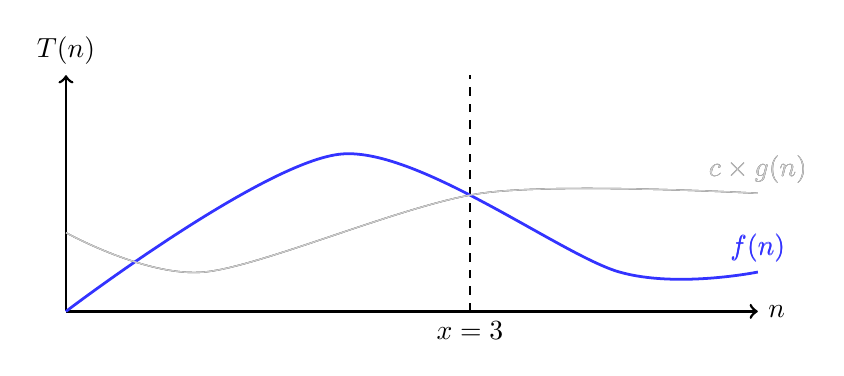
\begin{tikzpicture}[x=50]
            \draw<1->[->, line width=1] (0,0) -- (5,0) node[right] {$n$};
            \draw<1->[->, line width=1] (0,0) -- (0,3) node[above] {$T(n)$};

            % Curva preta
            \draw<3-4>[smooth, black!80, line width=0.5] plot coordinates
                {(0,1) (1,0.5) (3,1.5) (5, 1.5)} node[above] {$c\times g(n)$};
            % Curva azul forte
            \draw<2->[smooth, blue!80, line width=0.5] plot coordinates
                {(0,0) (2,2) (4,0.5) (5, 0.5)} node[above] {$f(n)$};
            % Assíntota
            \draw<4->[thin, dashed] (2.92, 0) node[below]
            {$x=3$} -- (2.92, 3);
            \draw<5->[smooth, blue!80, line width=1.0] plot coordinates
                {(0,0) (2,2) (4,0.5) (5, 0.5)} node[above] {$f(n)$};
            % Curva preta
            \draw<5->[smooth, black!20, line width=0.5] plot coordinates
                {(0,1) (1,0.5) (3,1.5) (5, 1.5)} node[above] {$c\times g(n)$};
        \end{tikzpicture}
    \end{center}
\end{frame}

\begin{frame}[fragile, t]
    \frametitle{Exemplo: Complexidade $O$}
    Verifique se o algoritmo é $O(n^2)$.\vfill

    \begin{lstlisting}[language=C++, basicstyle=\small]
      void funcao(int *v, int n){ 
        int soma = 0;
        for (int i=0; i<(n/2); i++) 
          for (int j=0; j<(n/4); j++) 
            soma += i + j;
        return soma;
      } 
  \end{lstlisting}\vfill

    \begin{columns}
        \begin{column}{0.4\textwidth}
            \begin{enumerate}
                \item[L2)] $1$
                \item[L3)] $1 + n/2$
                \item[L4)] $1 + (n/4)(n/2)$
                \item[L5)] $3(n/4)(n/2)$
                \item[L6)] $1$
            \end{enumerate}
        \end{column}
        \begin{column}{0.6\textwidth}
            \begin{align*}
                T(n) & = 4 + \left(\frac{n}{2}\right) + \left(\frac{n}{2}\frac{n}{4}\right) + 3\left(\frac{n}{2}\frac{n}{4}\right) \\
                T(n) & = 4 + \frac{n}{2}+ \frac{n^2}{2}
            \end{align*}

        \end{column}
    \end{columns}

\end{frame}

\begin{frame}[fragile, t]
    \frametitle{Exemplo: Complexidade O}
    $$T(n) = 4 + \frac{n}{2}+ \frac{n^2}{2} = \frac{8+n + n^2}{2}$$
    \begin{align*}
        0 & <f(n) \leq c\times g(n)                 \\
        0 & <\frac{8+n + n^2}{2} \leq c_1\times n^2
    \end{align*}

    A primeira inequação sempre será válida, basta então avaliar a segunda inequação:
    \begin{columns}
        \begin{column}{0.5\textwidth}
            \begin{align*}
                \frac{n^2 + n + 8}{2} & \leq c_1n^2  \\
                n^2 + n + 8           & \leq 2c_1n^2 \\
                n^2(1 - 2c_1) + n + 8 & \leq 0
            \end{align*}
        \end{column}
        \begin{column}{0.5\textwidth}
            Os valores de $c_1$ indicarão em quais condições $n$ permitirá que a inequação será verdadeira.
        \end{column}
    \end{columns}

\end{frame}

\begin{frame}[t]
    \frametitle{Análise de $n^2(1 - 2c_1) + n + 8 \leq 0$}
    Escolha de $c_1$:

    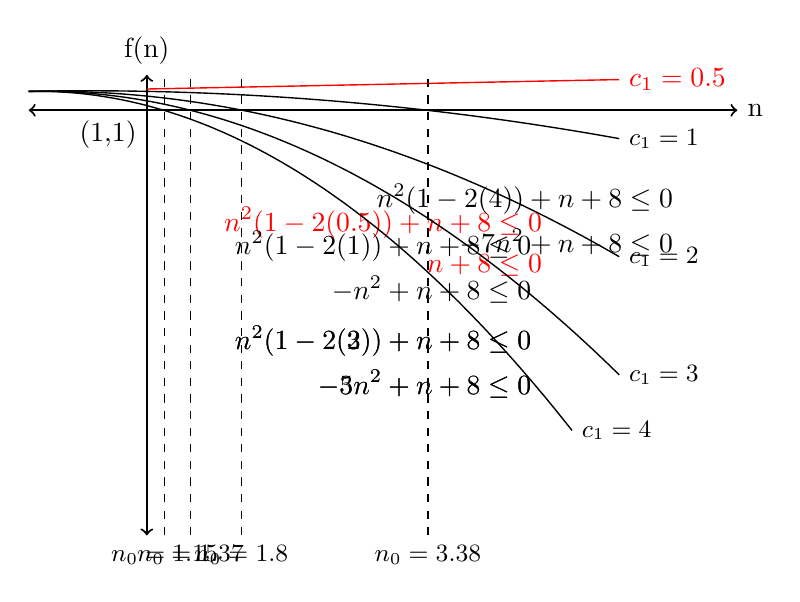
\begin{tikzpicture}[x=15mm, y=0.3mm]
        \draw[<->,line width=0.75pt] (0,0) -- (6,0) node[right] {n};
        \draw[<->,line width=0.75pt] (1,-180) -- (1,15) node[above] {f(n)};
        \draw[xshift=-14pt] (1,0.1) -- (1,-0.1) node[below] {(1,1)};
        \def\c_1{0.5}
        \draw<2>[domain=1:5, smooth=bezier, variable=\x, red,line width=0.5pt] plot ({\x},{(\x*\x)*(1-2*\c_1) + \x + 8}) node[right] {$c_1=0.5$};
        \node<2>[text width=150, color=red] at (3,-60) {
            \begin{align*}
                n^2 (1-2(0.5))+ n + 8 & \leq 0 \\
                n + 8                 & \leq 0
            \end{align*}};
        \def\c_1{1}
        \draw<3-5>[domain=0:5, smooth=bezier, variable=\x, black,line width=0.5pt] plot ({\x},{(\x*\x)*(1-2*\c_1) + \x + 8}) node[right] {\small$c_1=1$};
        \node<4>[text width=150] at (3,-60) {
            \begin{align*}
                n^2 (1-2(1))+ n + 8 & \leq 0 \\
                -n^2 + n + 8        & \leq 0
            \end{align*}};
        \draw<5>[-,line width=0.5pt, dashed] (3.38,-180) node[below] {\small$n_0 = 3.38$} -- (3.38,15);
        \def\c_1{2}
        \draw<6-8>[domain=0:5, smooth=bezier, variable=\x, black,line width=0.5pt] plot ({\x},{(\x*\x)*(1-2*\c_1) + \x + 8}) node[right] {\small$c_1=2$};
        \node<7>[text width=150] at (3,-100) {
            \begin{align*}
                n^2 (1-2(2))+ n + 8 & \leq 0 \\
                -3n^2 + n + 8       & \leq 0
            \end{align*}};
        \draw<8>[-,line width=0.5pt, dashed] (1.8,-180) node[below] {\small$n_0 = 1.8$} -- (1.8,15);
        \def\c_1{3}
        \draw<9-11>[domain=0:5, smooth=bezier, variable=\x, black,line width=0.5pt] plot ({\x},{(\x*\x)*(1-2*\c_1) + \x + 8}) node[right] {\small$c_1=3$};
        \node<10>[text width=150] at (3,-100) {
            \begin{align*}
                n^2 (1-2(3))+ n + 8 & \leq 0 \\
                -5n^2 + n + 8       & \leq 0
            \end{align*}};
        \draw<11>[-,line width=0.5pt, dashed] (1.37,-180) node[below] {\small$n_0 = 1.37$} -- (1.37,15);
        \def\c_1{4}
        \draw<12-14>[domain=0:4.6, smooth=bezier, variable=\x, black,line width=0.5pt] plot ({\x},{(\x*\x)*(1-2*\c_1) + \x + 8}) node[right] {\small$c_1=4$};
        \node<13>[text width=150] at (4.2,-40) {
            \begin{align*}
                n^2 (1-2(4))+ n + 8 & \leq 0 \\
                -7n^2 + n + 8       & \leq 0
            \end{align*}};
        \draw<14>[-,line width=0.5pt, dashed] (1.15,-180) node[below] {\small$n_0 = 1.15$} -- (1.15,15);
    \end{tikzpicture}

\end{frame}

\begin{frame}[t]
    \frametitle{Notação $\Omega$}
    Uma função $f(n)$ é dita como sendo $\Omega(g(n))$ se existe uma constante positivas $c$ para o qual:

    $$0< c\times g(n)\leq f(n)$$

    para todo $n>n_0$.

    \begin{center}
        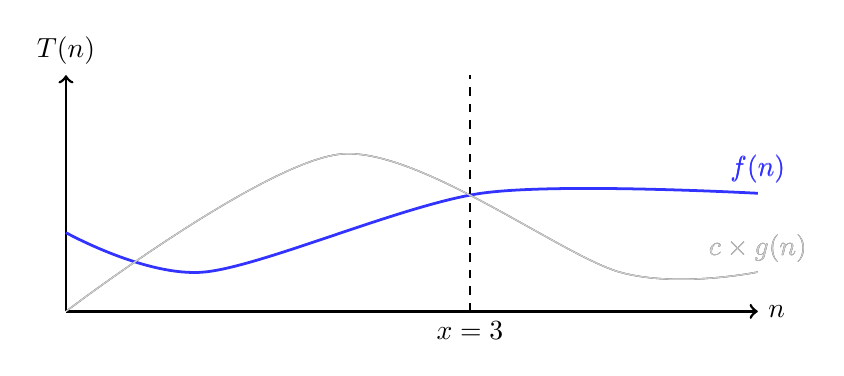
\begin{tikzpicture}[x=50]
            \draw<1->[->, line width=1] (0,0) -- (5,0) node[right] {$n$};
            \draw<1->[->, line width=1] (0,0) -- (0,3) node[above] {$T(n)$};

            % Curva preta
            \draw<3-4>[smooth, black!80, line width=0.5] plot coordinates
                {(0,0) (2,2) (4,0.5) (5, 0.5)} node[above] {$c\times g(n)$};
            % Curva azul forte
            \draw<2->[smooth, blue!80, line width=0.5] plot coordinates
                {(0,1) (1,0.5) (3,1.5) (5, 1.5)} node[above] {$f(n)$};
            % Assíntota
            \draw<4->[thin, dashed] (2.92, 0) node[below]
            {$x=3$} -- (2.92, 3);
            \draw<5->[smooth, blue!80, line width=1.0] plot coordinates
                {(0,1) (1,0.5) (3,1.5) (5, 1.5)}   node[above] {$f(n)$};
            % Curva preta
            \draw<5->[smooth, black!20, line width=0.5] plot coordinates
                {(0,0) (2,2) (4,0.5) (5, 0.5)}node[above] {$c\times g(n)$};
            % \draw[smooth, blue!80, line width=1] plot coordinates  
            %   {(0,1) (1,0.5) (3,1.5) (5, 1.5)} node[above] {$f(n)$};
        \end{tikzpicture}
    \end{center}
\end{frame}

\begin{frame}[t]
    \frametitle{Exemplo: Complexidade $\Omega$}

    Mostre que: $$2n^2 -20n -50\ \text{é}\ \Omega(2n)$$
    \vfill
    \hrule
    \vfill
    Resolvendo a inequação da notação $\Omega$:
    \begin{align}
        c_1\times (2n)          & \leq 2n^2 - 20n - 50 \\
        2n^2 - 20n - 50 - 2c_1n & \geq 0               \\
        2n^2 - n(20+2c_1) - 50  & \geq 0               \\
        n^2 - n(10+c_1) - 25    & \geq 0\label{eq4}
    \end{align}

    portanto, precisamos avaliar a concavidade desta curva. Escolher um valor de $c_1$ no qual a inequação~\ref{eq4} seja válida para qualquer valor de $n\geq n_0$.
\end{frame}

\begin{frame}[t]
    \frametitle{Exemplo: Complexidade $\Omega$}

    Ao analisar a inequação:

    $$n^2 - n(10+c_1) - 25    \geq 0$$

    Percebemos que se comporta como uma inequação do segundo grau no qual o produto e a soma das raízes são respectivamente $(10+c_1)$ e $(-25)$. Graficamente:

    \begin{center}

        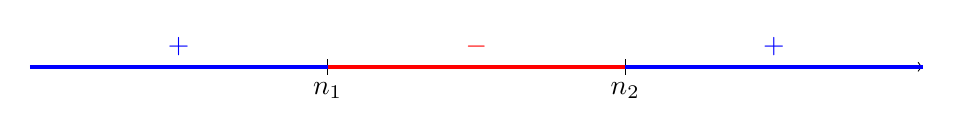
\begin{tikzpicture}[x=7mm]
            \draw[->] (0,0) -- (16.2,0);
            \draw[-] (5.4, -0.1) -- (5.4, 0.1) node[below, yshift=-5] {$n_1$};
            \draw[-] (10.8, -0.1) -- (10.8, 0.1) node[below, yshift=-5] {$n_2$};
            %   \node[anchor=east] at (n1) {+++++++++++++++++};
            %   \node[anchor=west] at (n1) {$-----------$};
            %   \node[anchor=west] at (n2) {+++++++++++++++};
            \draw[ultra thick, blue] (0,0) -- (5.4, 0) node[midway, above] {$+$};
            \draw[ultra thick, red] (5.4, 0) -- (10.8, 0) node[midway, above] {$-$};
            \draw[ultra thick, blue] (10.8, 0) -- (16.2, 0) node[midway, above] {$+$};

        \end{tikzpicture}
    \end{center}
    \begin{flushleft}
        \begin{columns}
            \begin{column}{0.45\textwidth}
                \begin{align*}
                    n_1 + n_2 & = 10+c_1 \\
                    n_1n_2    & = -25
                \end{align*}
                Escolhendo $c_1=2$, observamos que $n_1 \approx -13.81$ e $n_2 \approx -1.81$.
            \end{column}
            \begin{column}{0.45\textwidth}
                Ou seja:

                A partir de $n_0=2$, escolhendo $c_1=2$, a inequação será sempre válida.
            \end{column}
        \end{columns}
    \end{flushleft}
\end{frame}

\begin{frame}[t]
    \frametitle{Notação $\Theta$}
    Uma função $f(n)$ é dita como sendo $\Theta(g(n))$ se existem constantes positivas $c_1$, $c_2$ e $n_0$ para os quais:

    $$0<c_1g(n) \leq f(n)\leq c_2g(n)$$

    para todo $n>n_0$.

    \begin{center}
        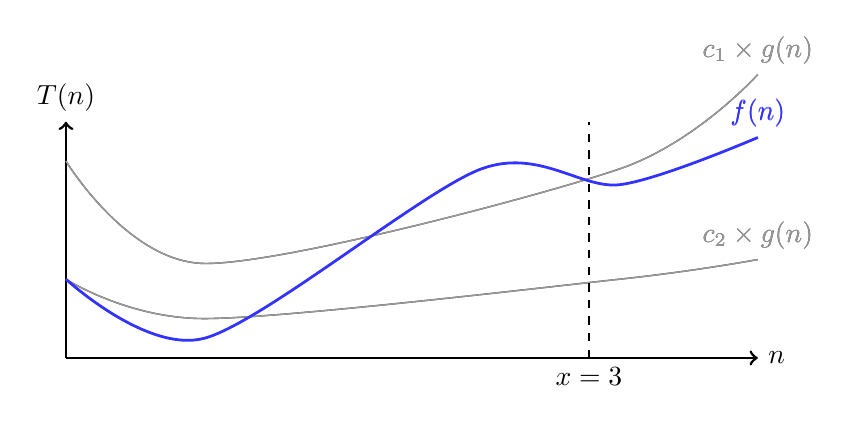
\begin{tikzpicture}[x=50]
            % Eixo x
            \draw<1->[->, line width=1] (0,0) -- (5,0) node[right] {$n$};
            \draw<1->[->, line width=1] (0,0) -- (0,3) node[above] {$T(n)$};
            \draw<2-4>[smooth, black!80, line width=0.5] plot coordinates {(0,2.5) (1,1.2) (4,2.4) (5, 3.6)} node[above] {$c_1\times g(n)$};
            \draw<3-4>[smooth, black!80, line width=0.5] plot coordinates {(0,1) (1,0.5) (4,1) (5, 1.25)} node[above] {$c_2\times g(n)$};
            \draw<4->[smooth, blue!80, line width=0.5] plot coordinates  {(0,1) (1,0.25) (3,2.4) (4, 2.2) (5, 2.8)} node[above] {$f(n)$};
            \draw<5->[smooth, black!40, line width=0.5] plot coordinates {(0,2.5) (1,1.2) (4,2.4) (5, 3.6)} node[above] {$c_1\times g(n)$};
            \draw<5->[smooth, black!40, line width=0.5] plot coordinates {(0,1) (1,0.5) (4,1) (5, 1.25)} node[above] {$c_2\times g(n)$};
            \draw<5->[smooth, blue!80, line width=1] plot coordinates  {(0,1) (1,0.25) (3,2.4) (4, 2.2) (5, 2.8)} node[above] {$f(n)$};
            \draw<5->[thin, dashed] (3.78, 0) node[below] {$x=3$} -- (3.78, 3);
        \end{tikzpicture}
    \end{center}
\end{frame}


\begin{frame}[t]
    \frametitle{Exemplo: Complexidade $\Theta$}

    Verifique se:

    $$\lg n\ \text{é}\ \Theta(\log_{10} n)$$

    Para ser $\Theta(\log_{10} n)$, a seguinte inequação deverá ser válida para um $c_1$ e $c_2$ positivos escolhidos arbitrariamente.

    $$0<c_1\log_{10}n \leq \lg{n}\leq c_2g(n)\log_{10}$$

    Devemos então resolver separadamente estas inequações sabendo que: $$\log_{10}n = \frac{\lg{n}}{\lg{10}}$$

\end{frame}


\begin{frame}[t]
    \frametitle{Exemplo: Complexidade $\Theta$}
    \begin{columns}
        \begin{column}{0.5\textwidth}
            Parte 1:
            $$c_1\log_{10}n \leq \lg{n}$$
            \begin{align*}
                c_1\frac{\lg{n}}{\lg{10}} & \leq \lg{n}  \\
                c_1                       & \leq \lg{10}
            \end{align*}
        \end{column}
        \begin{column}{0.5\textwidth}
            Parte 2:
            $$\lg{n} \leq c_2\log_{10}n $$
            \begin{align*}
                \lg{n} & \leq c_2\frac{\lg{n}}{\lg{10}} \\
                c_2    & \geq \lg{10}
            \end{align*}
        \end{column}
    \end{columns}
    \pause Ou seja, podemos escolher os valores:
    \begin{align*}
        c_1 = 2 & \leq \lg 10 \\
        c_2 = 3 & \geq \lg 10
    \end{align*}

    \pause Deste modo, a partir de $n_0 > 0$\footnote{Verifique esta afirmação}:

    $$0<c_1\log_{10}n \leq \lg{n}\leq c_2\log_{10}n$$


\end{frame}

\begin{frame} % Criação do frame
    \frametitle{Exemplo: Complexidade $\Theta$}
    \begin{center}

        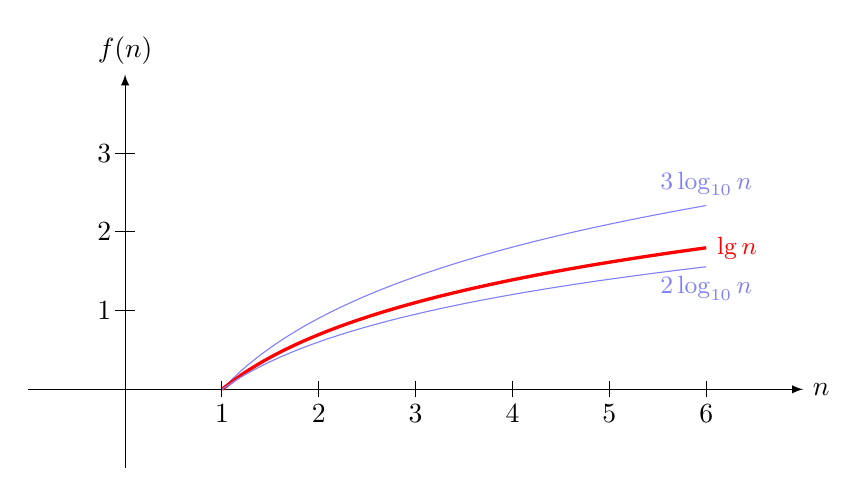
\begin{tikzpicture}[x=35]
            % Eixos
            \draw[-latex] (-1,0) -- (7,0) node[right] {$n$};
            \draw[-latex] (0,-1) -- (0,4) node[above] {$f(n)$};

            % Linha do gráfico
            \draw<1->[domain=1:6,smooth,variable=\x,blue!50] plot ({\x},{3*log10(\x)}) node[above] {\small$3\log_{10} n$};
            \draw<3->[domain=1:6,smooth,variable=\x,red, very thick] plot ({\x},{log10(\x)/log10(2.71)})node[right] {\small$\lg n$};
            \draw<2->[domain=1:6,smooth,variable=\x,blue!50] plot ({\x},{2*log10(\x)}) node[below] {\small$2\log_{10} n$};

            % Marcações nos eixos
            \foreach \x in {1,...,6}
            \draw (\x,-0.1) -- (\x,0.1) node[below, yshift=-5] {\x};
            \foreach \y in {1,...,3}
            \draw (-0.1,\y) -- (0.1,\y) node[left, xshift=-5] {\y};

        \end{tikzpicture}

    \end{center}

\end{frame}

\begin{frame}
    \begin{center}
        \frametitle{Ordem de Complexidade}
        \begin{tabular}{l|c}
            \textbf{Complexidade} & \textbf{Descrição simplificada} \\[5pt]
            \hline
            \pause $O(1)$         & Complexidade Constante          \\[5pt]
            \pause $O(log(n))$    & Complexidade logarítmica        \\[5pt]
            \pause $O(n)$         & Complexidade Linear             \\[5pt]
            \pause $O(n\ log(n))$ & Complexidade Log Linear         \\[5pt]
            \pause $O(n^2)$       & Complexidade Quadrática         \\[5pt]
            \pause $O(n^3)$       & Complexidade Cúbica             \\[5pt]
            \pause $O(2^n)$       & Complexidade Exponencial        \\[5pt]
            \pause $O(n!)$        & Complexidade Fatorial           \\[5pt]
        \end{tabular}
    \end{center}
\end{frame}


\begin{frame}[fragile, t]
    \frametitle{Complexidade Constante}
    \begin{itemize}
        \item Ocorre quando a complexidade do algoritmo independe do tamanho do problema (n);
        \item As instruções são executadas em uma quantidade fixa de vezes.
    \end{itemize}
    \pause Exemplo:
    \begin{lstlisting}[language=C++, basicstyle=\small]
        int funcConstante(int *v, int n){ 
          if(V[0] > V[n-1]){
            return V[n-1];
          }else{
            return V[0];
          }
        } 
    \end{lstlisting}

\end{frame}

\begin{frame}[fragile, t]
    \frametitle{Complexidade Logarítmica}
    \begin{itemize}
        \item Ocorre quando um problema é subdividido em em subproblemas menores.
        \item A solução deve ser apenas uma das soluções menores.
    \end{itemize}
    \pause Exemplo:
    \begin{lstlisting}[language=C++, basicstyle=\small]
        bool funcLog(int v[], int a, int b, int x)
        {
            if (a > b)
                return false;
            int c = (a + b) / 2;
            if (v[c] == x)
                return true;
            else if (v[c] > x)
                return funcLog(v, a, c-1, x);
            else
                return funcLog(v, c+1, b, x);
        }
    \end{lstlisting}

\end{frame}


\begin{frame}[fragile, t]
    \frametitle{Complexidade Linear}
    \begin{itemize}
        \item Ocorre quando a complexidade do algoritmo é proporcional ao tamanho do problema;
        \item O tempo computacional é um múltiplo de $n$ podendo ser acrescido de alguma constante.
    \end{itemize}
    \pause Exemplo:
    \begin{lstlisting}[language=C++, basicstyle=\small]
        int funcLinear(int *v, int n){ 
          int maior = v[0];
          int cont = 0;
          while(cont < n){
            if(v[cont] > maior){
                maior = v[i];
            }
            cont = cont + 1;
          }
          return maior;
        } 
    \end{lstlisting}

\end{frame}

\begin{frame}[fragile, t]
    \frametitle{Complexidade LogLinear}
    \begin{itemize}
        \item Ocorre quando o problema é subdividido em subproblemas;
        \item A solução será a união das contribuiçoes das resoluções dos subproblemas.
    \end{itemize}
    \pause Exemplo:
    \begin{lstlisting}[language=C++, basicstyle=\small]
        void funcLogLinear (int inicio, int fim){
            if ( inicio < fim ){
                int meio = ( inicio + fim )/2;
                funcLogLinear ( inicio , meio );
                funcLogLinear ( meio +1 , fim );
                unir ( inicio , meio , fim );
            }
         }
    \end{lstlisting}

\end{frame}
\begin{frame}[fragile, t]
    \frametitle{Complexidade Quadrática}
    \begin{itemize}
        \item Geralmente está associado a \textbf{dois laços} que são proporcionais ao tamanho do problema.
        \item Qualquer uma outra complexidade anterior pode ser adicionada sem mudança na complexidade quadrática.
    \end{itemize}
    \pause Exemplo:
    \begin{lstlisting}[language=C++, basicstyle=\small]
        void funcQuadratica (int *v, int n){
            int aux;
            for(int i=0; i<n; i++)
                for(int j=i+1; j<n; j++)
                    if(v[i] > V[j]){
                        aux = v[i];
                        v[i] = v[j];
                        v[j] = aux;
                    }
         }
    \end{lstlisting}

\end{frame}

\begin{frame}[fragile, t]
    \frametitle{Complexidade Cúbica}
    \begin{itemize}
        \item Geralmente está associado a \textbf{três laços} que são proporcionais ao tamanho do problema.
        \item Qualquer uma outra complexidade anterior pode ser adicionada sem mudança na complexidade Cúbica.
    \end{itemize}
    \pause Exemplo:
    \begin{lstlisting}[language=C++, basicstyle=\small]
        void funcCubica (int *v, int n){
            int aux;
            for(int i=0; i<n; i++)
                for(int j=i+1; j<n; j++)
                    for(int k=j+1; j<n; j++)
                        aux = v[i] + v[j] + v[k];
                        printf("%d", aux);
         }
    \end{lstlisting}

\end{frame}

\begin{frame}[fragile, t]
    \frametitle{Complexidade Exponencial ($2^n$)}
    \begin{itemize}
        \item Geralmente está associado a um problema que a resolução é feita por \textbf{força-bruta}.
        \item Qualquer uma outra complexidade anterior pode ser adicionada sem mudança na complexidade Exponencial.
    \end{itemize}
    \pause Exemplo:
    \begin{lstlisting}[language=C++, basicstyle=\small]
        int funcExp(int n){
            int aux;
            if(n < 2)
                return n;
            else
                return funcExp(n-1) + funcExp(n-2);
         }
    \end{lstlisting}

    \pause\textbf{Exercício}: Prove se é verdadeiro ou falso:

    $$f(n) = 3^n\ \text{é}\ O(2^n)$$

\end{frame}

\begin{frame}[fragile, t]
    \frametitle{Complexidade Fatorial ($n!$)}

    \begin{itemize}
        \item Complexidade para algoritmo de força-bruta;
        \item Problemas como caixeiro-viajante e criptografia podem se valer desta complexidade.
    \end{itemize}

\end{frame}
\begin{frame}[fragile,t]
    \frametitle{Pior, Melhor e Caso médio}

    Considere p algoritmo abaixo:

    \begin{lstlisting}[language=C++, basicstyle=\small]
        #define N 100000
        int busca(int *A, int v){
            for(int x = 0; x<N; x++){
                if(A[x] == v)
                    return x;
            }
            return -1;
        }
    \end{lstlisting}
    \vfill
    \begin{itemize}
        \item Como avaliar esse algoritmo?
        \item O desempenho depende apenas do tamanho de N?
        \item O desempenho é modificado pelos valores de entrada?
    \end{itemize}
\end{frame}

\begin{frame}[t]
    \frametitle{Pior, Melhor e Caso médio}
    \begin{itemize}
        \item \textbf{Pior caso} é a função que relaciona o tamanho da entrada $n$ com o maior tempo possível para execução deste problema.
        \item \textbf{Melhor caso} é a função que relaciona o tamanho da entrada $n$ com o menor tempo possível para execução deste problema.
        \item \textbf{Caso médio} é a função que relaciona o tamanho da entrada $n$ com o tempo médio para execução deste problema. Para isso, é considerado uma \emph{distribuição de probabilidade} das possíveis entradas.
    \end{itemize}

\end{frame}

\begin{frame}[fragile, t]
    \frametitle{Exemplo: }
    Qual o pior, melhor e o caso médio para a execução desse algoritmo? Quais suas complexidades?

    \begin{lstlisting}[language=C++, basicstyle=\small]
        #define N 100000
        int busca(int *A, int v){
            for(int x = 0; x<N; x++){
                if(A[x] == v)
                    return x;
            }
            return -1;
        }
    \end{lstlisting}
\end{frame}

\begin{frame}
    \frametitle{Exemplo: Complexidade média}
    Considere:
    \begin{itemize}
        \item $0\leq p\leq 1$ é a probabilidade de \emph{v} estar no vetor \emph{A};
        \item $p/n$ é a probabilidade de $v$ estar no vetor \emph{A} na posição $x$.
    \end{itemize}

    \pause Desta forma, podemos dizer que:
    \begin{itemize}
        \item O custo de encontrar um elemento é:
              \begin{align}\label{Eq1}
                  1\times \frac{p}{n} + 2\times \frac{p}{n} +\ldots n\times \frac{p}{n}= \pause \sum_{i=1}^n i\times \frac{p}{n}
              \end{align}
              \item O custo do elemento não ser encontrado é:
              \begin{align}\label{Eq2}
                  (1-p) (n+1)
              \end{align}
    \end{itemize}
\end{frame}

\begin{frame}
    \frametitle{Exemplo: Complexidade média}
    Somando \ref{Eq2} com \ref{Eq1}, temos:

    \begin{align*}
        S_{medio} & = (1-p) (n+1) + \sum_{i=1}^n i*\frac{p}{n}  \\
                  & = (1-p)(n+1) + \frac{p}{n} \sum_{i=1}^n i   \\
                  & = (1-p)(n+1) + \frac{p}{n} \frac{n(n+1)}{2} \\
                  & = \frac{(n+1)(2-p)}{2}                      \\
    \end{align*}

    \begin{itemize}
        \item Considere $p=1$ (busca bem sucedida), então o custo médio será de $\frac{n+1}{2}$.
        \item Considere $p=0$ (busca mal sucedida), então o custo médio será de $(n+1)$.
    \end{itemize}
\end{frame}


\begin{frame}
    \frametitle{Considerações sobre complexidades}

    Pontos importantes:

    \begin{itemize}
        \item A complexidade \textbf{média} é de mais difícil obtenção: Dificuldade maior na análise.
        \item A complexidade no \textbf{pior} caso é tão importante quanto por apresentar o pior cenário possível.
        \item A complexidade no \textbf{melhor} caso não é tão relevante para análise de algoritmos.
        \item A complexidade do caso médio \textbf{não} é a média entre o pior caso e o melhor caso.

    \end{itemize}
\end{frame}

\begin{frame}[t]
    \frametitle{Complexidades}
    Pior e Caso médio das estruturas básicas:
    \begin{table}[]
        \resizebox{10cm}{!}{%
            \begin{tabular}{p{3cm}|l|l|l|l}
                \textbf{Estrutura} & \textbf{$n^0$ elem} & \textbf{Busca} & \textbf{Inserção} & \textbf{Remoção} \\
                \hline
                Array              & $O(1)$                & $O(n)$           & $O(n)$              & $O(n)$             \\
                Pilha              & $O(n)$                & $O(n)$           & $O(1)$              & $O(1)$             \\
                Fila               & $O(n)$                & $O(n)$           & $O(1)$              & $O(1)$
            \end{tabular}%
        }
    \end{table}
\end{frame}

\begin{frame}[t]
    \frametitle{Complexidades}
    \begin{table}[h]
        \resizebox{0.8\textwidth}{!}{%
        \renewcommand{\arraystretch}{1.5}
        \begin{tabular}{l|c|c|c}
            \textbf{Algoritmo} & \textbf{Pior Caso} & \textbf{Caso Médio} & \textbf{Melhor Caso} \\
            \hline
            \pause Bubble Sort & $O(n^2)$ & $O(n^2)$ & $O(n)$ \\
            \pause Insertion Sort & $O(n^2)$ & $O(n^2)$ & $O(n)$ \\
            \pause Selection Sort & $O(n^2)$ & $O(n^2)$ & $O(n^2)$ \\
            \pause Merge Sort & $O(n \log n)$ & $O(n \log n)$ & $O(n \log n)$ \\
            \pause Heap Sort & $O(n \log n)$ & $O(n \log n)$ & $O(n \log n)$ \\
            \pause Quick Sort & $O(n^2)$ & $O(n \log n)$ & $O(n \log n)$ \\
            \pause Tree Sort & $O(n^2)$ & $O(n \log n)$ & $O(n \log n)$ \\
            \pause Counting Sort & $O(n + k)$ & $O(n + k)$ & $O(n + k)$ \\
            \pause Bucket Sort & $O(n^2)$ & $O(n^2)$ & $O(n + k)$ \\
            \pause Radix Sort & $O(nk)$ & $O(nk)$ & $O(nk)$ \\
        \end{tabular}}
    \end{table}
\end{frame}
\end{document}

